\section{Introduction}

Prediction of the future state of complex systems is integral to the functioning of our society.
Some of these systems include weather \cite{weather-violence2013}, health \cite{ginsberg2008detecting}, the economy \cite{sornette2006predictability}, marketing \cite{asur2010predicting} and engineering \cite{savely1972}.
For weather in particular, this prediction is made using supercomputers across the world in the form of numerical weather model integrations taking our current best guess of the weather into the future.
The accuracy of these predictions depend on the accuracy of the models themselves, and the quality of our knowledge of the current state of the atmosphere.

Model accuracy has improved with better meteorological understanding of weather processes and advances in computing technology.
To solve the initial value problem, techniques developed over the past 50 years are now broadly known as {\em data assimilation}.
Formally, data assimilation is the process of using all available information, including short-range model forecasts and physical observations, to estimate the current state of a system as accurately as possible \cite{yang2006}.

We employ a toy climate experiment as a testbed for improving numerical weather prediction algorithms, focusing specifically on data assimilation methods.
This approach is akin to the historical development of current methodologies, and provides a tractable system for rigorous analysis.
The experiment is a thermal convection loop, which by design simplifies our problem into the prediction of convection.
The dynamics of thermal convection loops have been explored under both periodic \cite{keller1966} and chaotic \cite{welander1967,creveling1975stability,gorman1984,gorman1986,ehrhard1990dynamical,yuen1999,jiang2003,burroughs2005reduced,desrayaud2006numerical,yang2006,ridouane2010} regimes.
A full characterization of the computational behaivor of a loop under flux boundary conditions by Louisos et. al. describes four regimes: chaotic convection with reversals, high Ra aperiodic stable convection, steady stable convection, and conduction/quasi-conduction \cite{louisos2013}.
For the remainder of this work, we focus on the chaotic flow regime.

Computational simulations of the thermal convection loop are performed with the open-source finite volume C++ library OpenFOAM \cite{jasak2007}.
The open-source nature of this software enables its integration with the data assimilation framework that this work provides.

\section{Physical Experiment and Computational Model}

The thermosyphon, a type of natural convection loop or non-mechanical heat pump, can be likened to a toy model of climate \cite{harris2011predicting}.
\begin{figure}[t!]
  \centering
  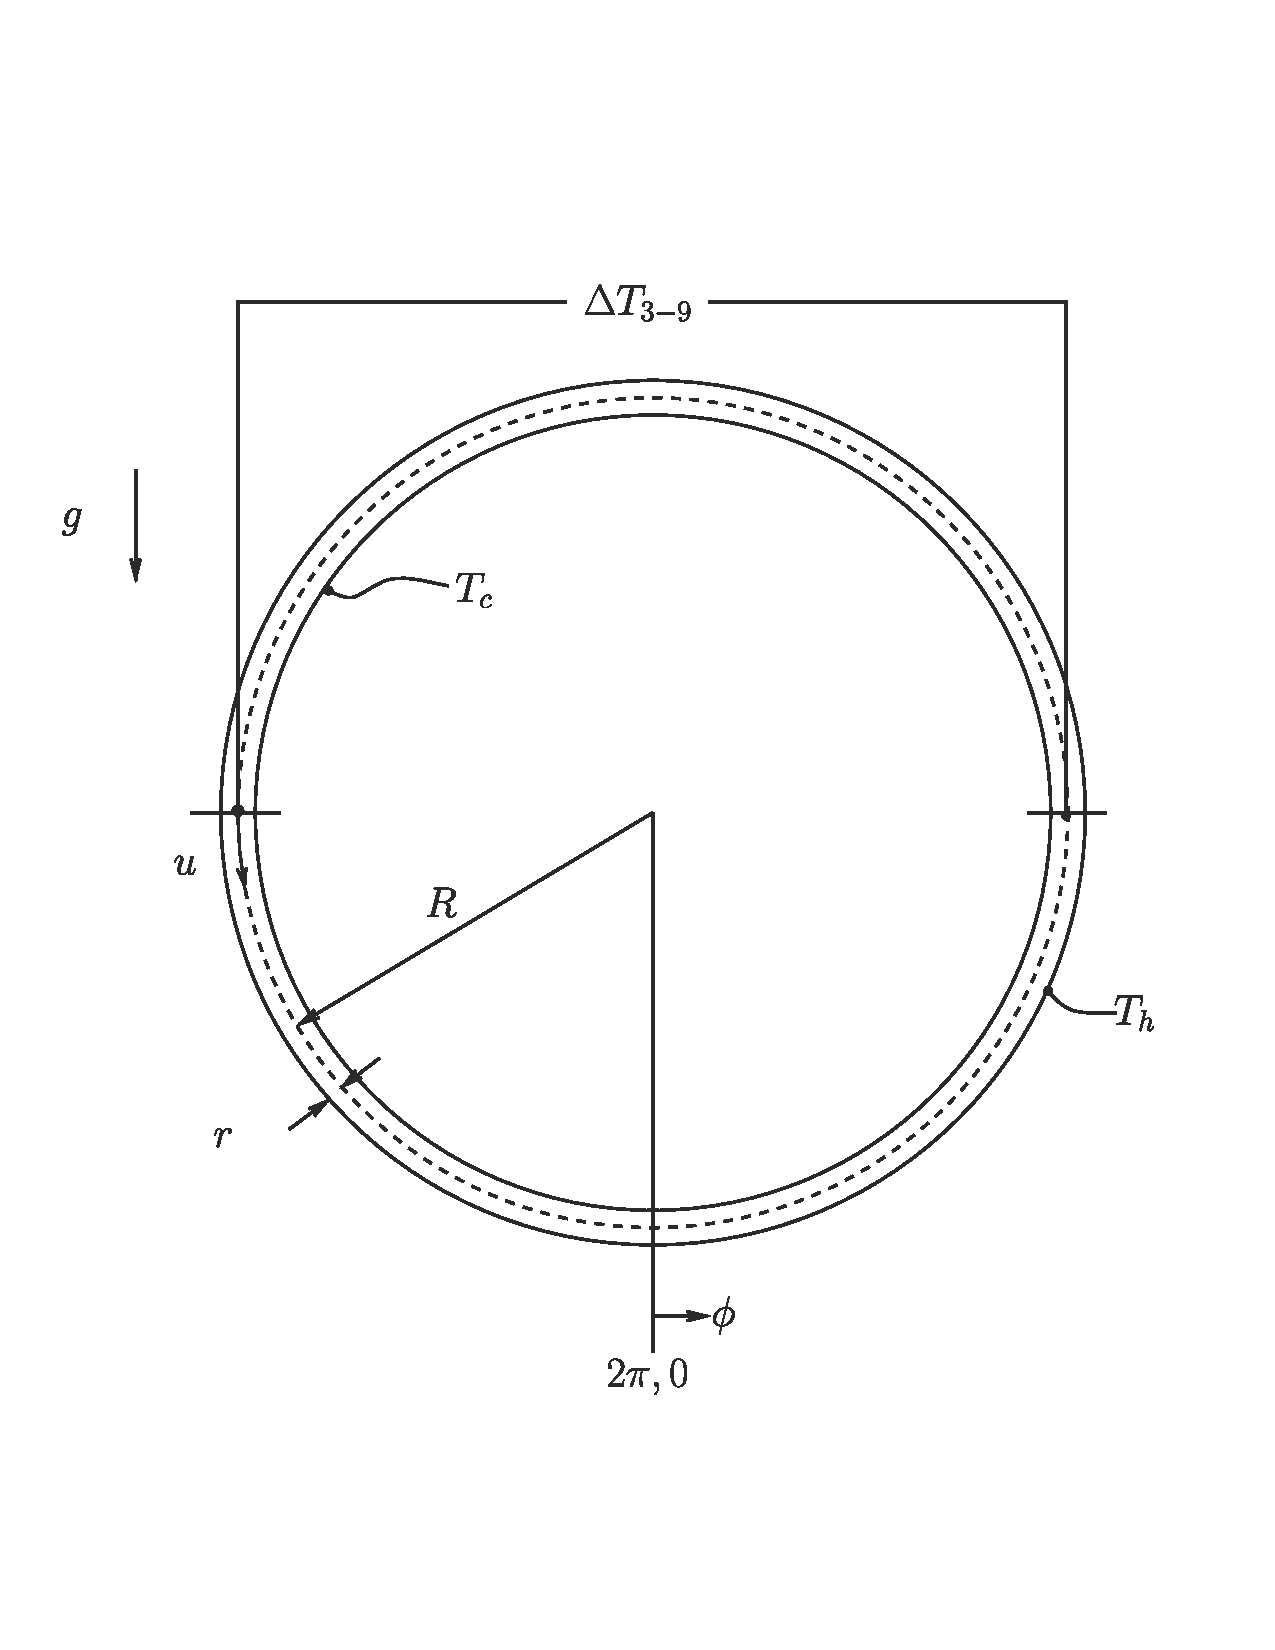
\includegraphics[width=0.45\textwidth]{figures/harris-tellus-2012-loop.pdf}
  \caption[Schematic of the experimental, and computational, setup from Harris et al (2012)]{
    Schematic of the experimental, and computational, setup from Harris et al (2012).
    The loop radius is given by $R$ and inner radius by $r$.
    The top temperature is labeled $T_c$ and bottom temperature $T_h$, gravity $g$ is defined downward, the angle $\phi$ is prescribed from the 6 o'clock position, and temperature difference $\Delta T_{3-9}$ is labeled.
  }
  \label{fig:thermosyphons}
\end{figure}

The reduced order system describing a thermal convection loop was originally derived by Gorman \cite{gorman1986} and Ehrhard and M\"{u}ller \cite{ehrhard1990dynamical}.
Here we present this three dimensional system in non-dimensionalized form.
In Appendix B we present a more complete derivation of these equations, following the derivation of Harris \cite{harris2011predicting}.
For $x_{\{1,2,3\}}$ the mean fluid velocity, temperature different $\Delta T_{3-9}$, and deviation from conductive temperature profile, respectively, these equations are:
\begin{align}
& \diff{x_1}{t} = \alpha (x_2 - x_1),\\
& \diff{x_2}{t} = \beta x_1 - x_2 (1 + Kh(|x_1|)) - x_1x_3,\\
& \diff{x_3}{t} = x_1x_2 - x_3 (1 + Kh(|x_1|)) .\end{align}
The parameters $\alpha$ and $\beta$, along with scaling factors for time and each model variable can be fit to data using standard parameter estimation techniques.

\begin{figure}[h!]
  \centering
  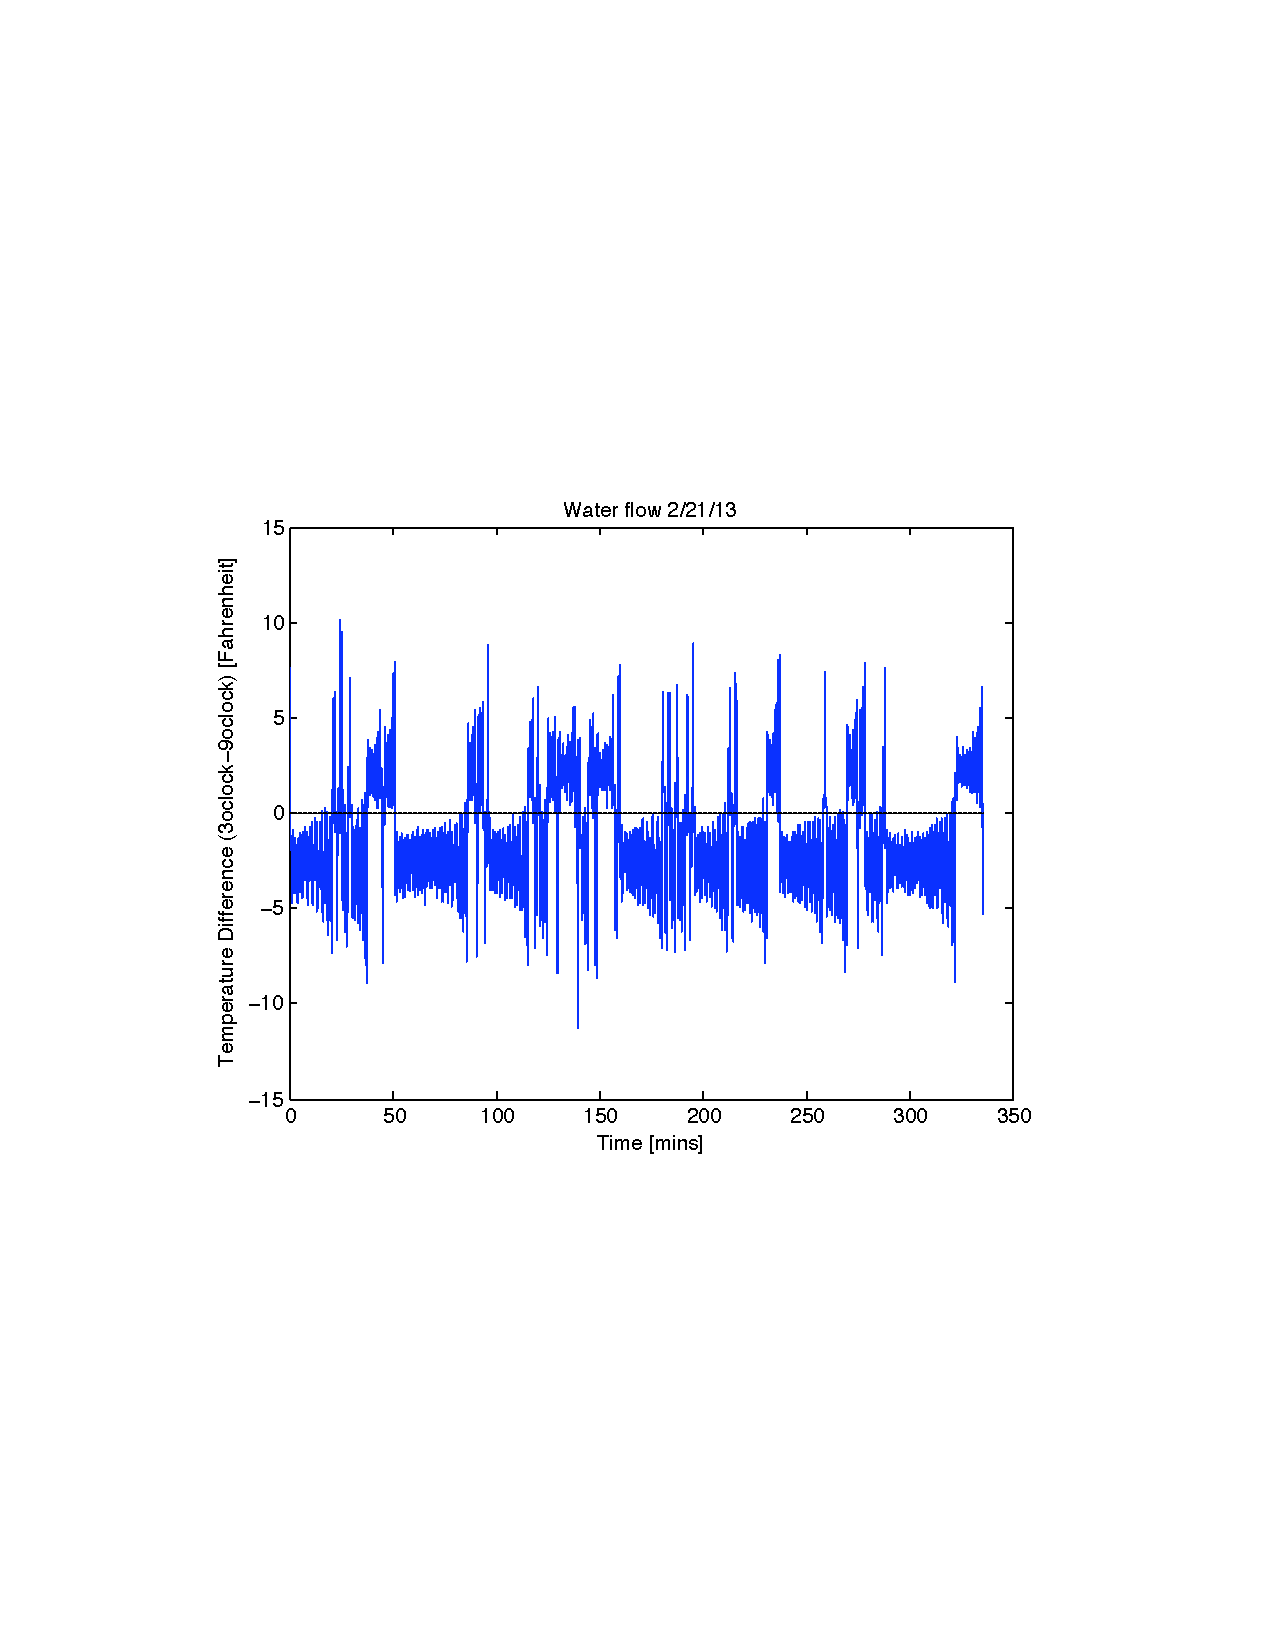
\includegraphics[width=0.45\textwidth]{figures/221TimeSeries.pdf}
  \caption[A time series of the physical thermosyphon, from the Undergraduate Honor's Thesis of Darcy Glenn {\protect \cite{glenn2013}}]{
    A time series of the physical thermosyphon, from the Undergraduate Honor's Thesis of Darcy Glenn {\protect \cite{glenn2013}}.
    The temperature difference (plotted) is taken as the difference between temperature sensors in the 3 and 9 o'clock positions.
    The sign of the temperature difference indicates the flow direction, where positive values are clockwise flow.
  }
  \label{fig:chrisLoop}
\end{figure}

%% \begin{figure}[h!]
%%   \centering
%%   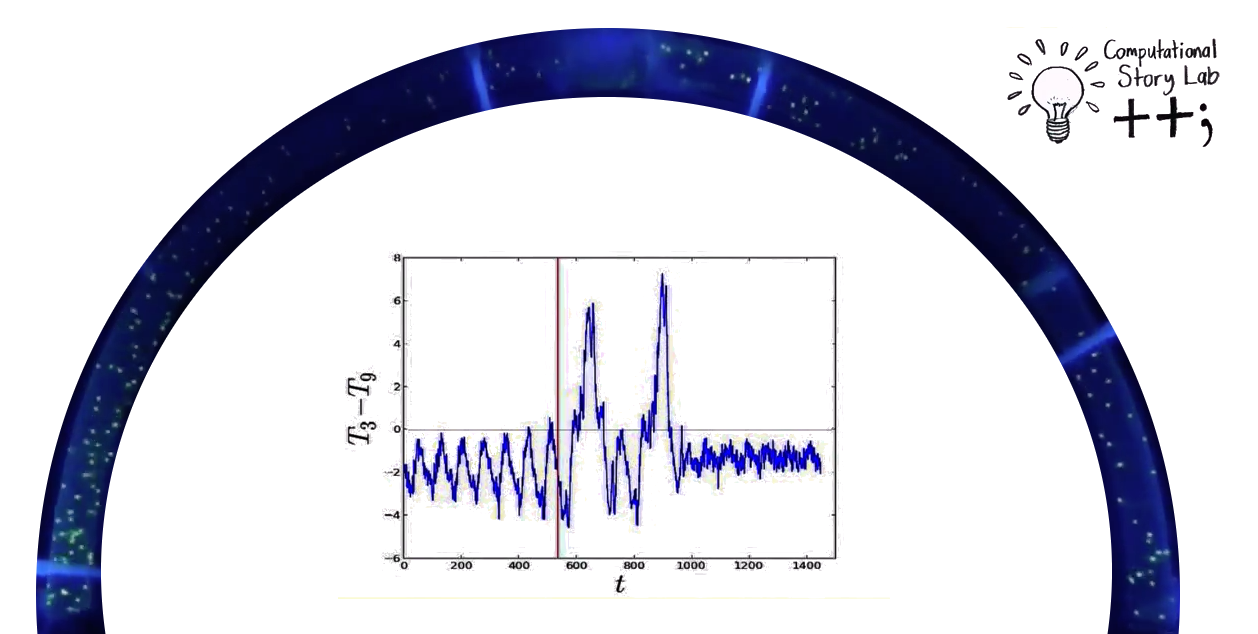
\includegraphics[width=0.45\textwidth]{figures/convectionLoopYoutubeScreenShot3.png}
%%   \caption[The Thermal Convection Loop experiment]
%%   {
%%     The Thermal Convection Loop experiment, inlaid with a time series of the temperature difference $\Delta T_{3-9}$ whose sign indicates the flow direction.
%%     Fluorescent balls are lit by a black-light and move with the flow.
%%     As the timeseries indicates, the flow changes direction aperiodically, giving rise to the chaotic behavior that we model.
%%     A video of the loop, from which this is a snapshot, can be viewed at \url{http://www.youtube.com/watch?feature=player_embedded&v=Vbni-7veJ-c}.
%%           }
%%   \label{fig:chrisLoop}
%% \end{figure}

Operated by Dave Hammond, UVM's Scientific Electronics Technician, the experimental thermosyphons access the chaotic regime of state space found in the principled governing equations.
We quote the detailed setup from Darcy Glenn's undergraduate thesis \cite{glenn2013}:
\begin{quote}
The [thermosyphon] was a bent semi-flexible plastic tube with a 10-foot heating rope wrapped around the bottom half of the upright circle.
The tubing used was light-transmitting clear THV from McMaster-Carr, with an inner diameter of 7/8 inch, a wall thickness of 1/16 inch, and a maximum operating temperature of 200F.
The outer diameter of the circular thermosyphon was 32.25 inches.
This produced a ratio of about 1:36 inner tubing radius to outside thermosyphon radius (Danforth 2001).
There were 1 inch 'windows' when the heating cable was coiled in a helix pattern around the outside of the tube, so the heating is not exactly uniform.
The bottom half was then insulated using aluminum foil, which allowed fluid in the bottom half to reach 176F.
A forcing of 57 V, or 105 Watts, was required for the heating cable so that chaotic motion was observed.
Temperature was measured at the 3 o'clock and 9 o'clock positions using unsheathed copper thermocouples from Omega.
\end{quote}
We first test our ability to predict this experimental thermosyphon using synthetic data, and describe the data in more detail in Chapter 4.
Synthetic data tests are the first step, since the data being predicted is generated by the predictive model.
We consider the potential of up to 32 synthetic temperature sensors in the loop, and velocity reconstruction from particle tracking, to gain insight into which observations will make prediction possible.

\subsection{Computational Setup}
We consider the incompressible Navier-Stokes equations with the Boussinesq approximation to model the flow of water inside a thermal convection loop.
For brevity, we omit the equations themselves, and include them in the Appendix.
The solver in OpenFOAM that we use, with some modification, is ``buoyantBoussinesqPimpleFoam.''
Solving is accomplished by the Pressure-Implicit Split Operator (PISO) algorithm \cite{issa1986solution}.
Modification of the code was necessary for laminar operation.

Both 2-dimensional and 3-dimensional meshes were created using OpenFOAM's native meshing utility ``blockMesh.''
After creating a mesh, we consider refining the mesh near the walls to capture boundary layer phenomena and renumbering the mesh for solving speed.
To refine the mesh near walls, we used the ``refineWallMesh'' utility, 
Lastly, the mesh is renumbered using the ``renumberMesh'' utility, which implements the Cuthill-McKee algorithm to minimize the adjacency matrix bandwidth, defined as the maximum distance from diagonal of nonzero entry.
The 2D mesh contains 40,000 points, and is imposed with fixed value boundary conditions on the top and bottom of the loop.

\begin{figure}[t!]
  \centering
  \includegraphics[width=0.45\textwidth]{/Users/andyreagan/work/2013/2013-05data-assimilation/OpenFOAM/figures/heating_zoom_mesh4.png}
  \caption[A snapshot of the mesh used for CFD simulations]{
  A snapshot of the mesh used for CFD simulations.
  Shown is an initial stage of heating for a fixed value boundary condition, 2D, laminar simulation with a mesh of 40000 cells including wall refinement with walls heated at 340K on the bottom half and cooled to 290K on the top half.
  }
  \label{fig:CFDmesh1}
\end{figure}

\begin{figure}[t!]
  \centering
  \includegraphics[width=0.45\textwidth]{/Users/andyreagan/work/2013/2013-05data-assimilation/OpenFOAM/figures/3D-mesh2.png}
  \caption[The 3D mesh viewed as a wireframe from within]{
  The 3D mesh viewed as a wireframe from within.
  Here there are 900 cells in each slice (not shown), for a total mesh size of 81,000 cells.
  Simulations using this computational mesh are prohibitively expensive for use in a real time ensemble forecasting system, but are possible offline.
  }
  \label{fig:CFDmesh2}
\end{figure}

Available boundary conditions (BCs) that were found to be stable in OpenFOAM's solver were constant gradient, fixed value conditions, and turbulent heat flux.
Simulations with a fixed flux BC is implemented through the externalWallHeatFluxTemperature library were unstable and resulted in physically unrealistic results.
Constant gradient simulations were stable, but the behavior was empirically different from our physical system.
To most accurately model our experiment, we choose a fixed value BC.
This is acceptable due to the thermal diffusivity and thickness of the walls of the experimental setup.

With the mesh, BCs, and solver chosen, we now simulate the flow.
From the data of $T,\phi,u,v,w$ and $p$ that are saved at each timestep, we extract the mass flow rate and average temperature at the $12,3,6$ and $9$ o'clock positions on the loop.
Since $\phi$ is saved as a face-value flux, we compute the mass flow rate over the cells $i$ of top (12 o'clock) slice as
\begin{equation} \sum _i\phi_{f(i)} \cdot v_i \cdot \rho_i\end{equation}
where $f(i)$ corresponds the face perpendicular to the loop angle at cell $i$ and $\rho$ is reconstructed from the Boussinesq approximation $\rho = \rhoref (1-\beta(T-T_\text{ref}))$.

Here is a picture of the thermosyphon colored by temperature.
\begin{figure}[h!]
  \centering
  \includegraphics[width=0.45\textwidth]{/Users/andyreagan/work/2013/2013-05data-assimilation/OpenFOAM/figures/heating003.png}
  \caption[A screenshot of the whole simulated loop]{
  A screenshot of the whole computationally simulated loop.
  Shown is an initial stage of heating for a fixed value boundary condition, 2D, laminar simulation with a mesh of 40000 cells including wall refinement with walls heated at 340K on the bottom half and cooled to 290K on the top half.
  Note that the colorbar limits are truncated to allow for visualization of the dynamics far from the boundary.
  }
  \label{fig:CFDloopSS}
\end{figure}




\section{Data Assimilation Methods}

Tests of the data assimilation algorithms described here are performed with the Lorenz 63 system, which is analogous to the above equations with Lorenz's $\beta = 1$, and $K = 0$.
The cannonical choice of $\sigma = 10, \beta = 8/3$ and $\rho = 28$, produce the well known butterfly attractor, is used for all examples here.
From these tests, we have found the optimal data assimilation parameters (inflation factors) for predicting time-series with this system.
We focus our efforts on making prediction using computational fluid dynamics models.

We first implement the 3D-Var filter.
Simply put, 3D-Var is the variational (cost-function) approach to finding the analysis.
It has been shown that 3D-var solves the same statistical problem as OI \cite{lorenc1986analysis}.
The usefulness of the variational approach comes from the computational efficiency, when solved with an iterative method.
The multivariate 3D-Var is thus finding the $\mbx _a$ that minimizes the cost function
\begin{equation} J(\mbx) = (\mbx - \mbx_b) ^T \mbB ^{-1} (\mbx - \mbx_b) + (\mby_o + H(\mbx))^T\mbR (\mby_o - H(\mbx)) .\end{equation}

Next, we implemented the ``gold-standard'' Extended Kalman Filter (EKF).
The TLM is precisely the model (written as a matrix) that transforms a perturbation at time $t$ to a perturbation at time $t+\Delta t$, analytically equivalent to the Jacobian of the model.
Using the notation of Kalnay \cite{kalnay2003}, this amounts to making a forecast with the nonlinear model $M$, and updating the error covariance matrix $\mbP$ with the TLM $L$, and adjoint model $L^T$

\begin{align*} \mbx^f (t_i) &= M _{i-1} [\mbx ^a (t_{i-1} ) ]\\
\mbP^f (t_i ) &= L_{i-1} \mbP^a (t_{i-1} ) L^T _{i-1} + \mathbf{Q} (t_{i-1} ) \end{align*}

where $\mathbf{Q}$ is the noise covariance matrix (model error).
In the experiments with Lorenz 63 presented in this section, $\mathbf{Q} = 0$ since our model is perfect.
In NWP, $\mathbf{Q}$ must be approximated, e.g. using statistical moments on the analysis increments \cite{danforth2007estimating,li2009accounting}.

The analysis step is then written as (for $H$ the observation operator):
\begin{align} \mbx^a (t_i ) &= \mbx^f (t_i) + \mbK_i \mbd_i\\
\mbP^a (t_i) &= (\mathbf{I} - \mbK_i \mbH_i )\mbP^f (t_i) \end{align}
where
\[ \mbd_i = \mby_i^o - \mbH[x^f (t_i) ] \]
is the innovation. The Kalman gain matrix is computed to minimize the analysis error covariance $P^a _i$ as
\[ \mbK_i = \mbP^f (t_i) \mbH_i ^T [ \mbR_i + \mbH_i \mbP^f (t_i) \mbH^T ] ^{-1} \]
where $\mbR_i$ is the observation error covariance.
Since we are making observations of the truth with random normal errors of standard deviation $\mbe$, the observational error covariance matrix $\mbR$ is a diagonal matrix with $\epsilon$ along the diagonal.
The most difficult, and most computationally expensive, part of the EKF is deriving and integrating the TLM.
For this reason, the EKF is not used operationally, and later we will turn to statistical approximations of the EKF using ensembles of model forecasts.
Next, we go into more detail regarding the TLM.

The TLM is the model which advances an initial perturbation $\delta \mbx_{i}$ at timestep $i$ to a final perturbation $\delta \mbx_{i+1}$ at timestep $i+1$.
The dynamical system we are interested in, Lorenz '63, is given as a system of ODE's:
\[ \frac{d\mbx}{dt} = F(\mbx) .\]
We integrate this system using a numerical scheme of our choice (in the given examples we use a second-order Runge-Kutta method), to obtain a model $M$ discretized in time.
\[ \mbx(t) = M[ \mbx(t_0) ] .\]
Introducing a small perturbation $\mby$, we can approximate our model $M$ applied to $\mbx(t_0) + \mby(t_0)$ with a Taylor series around $\mbx(t_0)$:
\begin{align*} M[ \mbx(t_0) + \mby(t_0) ] &= M [ \mbx(t_0) ] + \frac{\partial M}{\partial \mbx} \mby(t_0) + O [ \mby(t_0) ^2 ]\\ &\approx \mbx(t) + \frac{\partial M}{\partial \mbx} \mby(t_0) .\end{align*}
We can then solve for the linear evolution of the small perturbation $\mby(t_0)$ as 
\begin{equation} \frac{d\mby }{dt } = \mathbf{J} \mby \label{eq:ODETLM} \end{equation}
where $\mathbf{J} = \partial F / \partial \mbx$ is the Jacobian of $F$.
We can solve the above system of linear ordinary differential equations using the same numerical scheme as we did for the nonlinear model.
To verify our implementation of the TLM, we propagate a small error in the Lorenz 63 system and plot the difference between that error and the TLM predicted error, for each variable (Figure \ref{fig:TLMverification}).

\begin{figure}[h!]
  \centering
  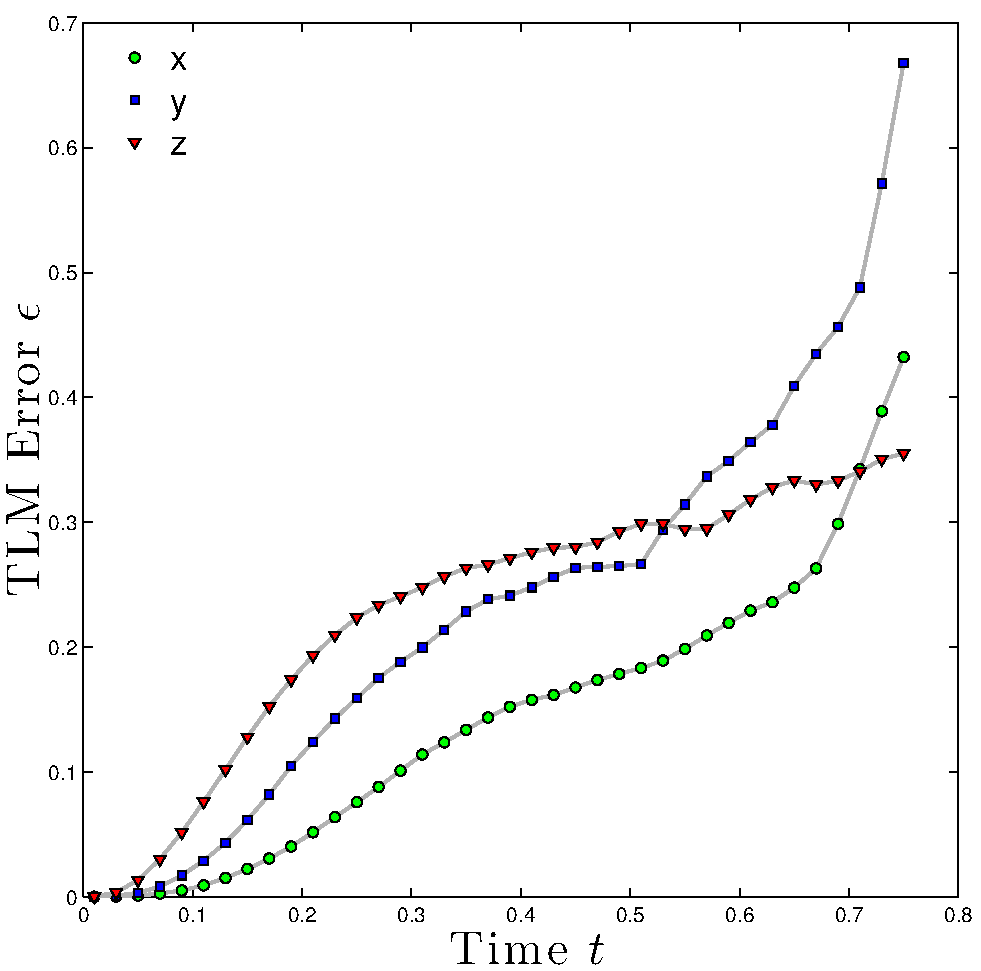
\includegraphics[width=0.45\textwidth]{figures/TLM-verification003_noname.pdf}
  \caption[The future error predicted by the TLM is compared to the error growth in Lorenz 63 system for an initial perturbation with standard deviation of 0.1, averaged over 1000 TLM integrations]{
    The future error predicted by the TLM is compared to the error growth in Lorenz 63 system for an initial perturbation with standard deviation of 0.1, averaged over 1000 TLM integrations.
    The $\epsilon$ is not the error predicted by the TLM, but rather the error of the TLM in predicting the error growth.
  }
  \label{fig:TLMverification}
\end{figure}

The computational cost of the EKF is mitigated through the approximation of the error covariance matrix $\mbP_f$ from the model itself, without the use of a TLM.
One such approach is the use of a forecast ensemble, where a collection of models (ensemble members) are used to statistically sample model error propagation.
With ensemble members spanning the model analysis error space, the forecasts of these ensemble members are then used to estimate the model forecast error covariance.
%% \begin{figure}[h!]
%%   \centering
%%   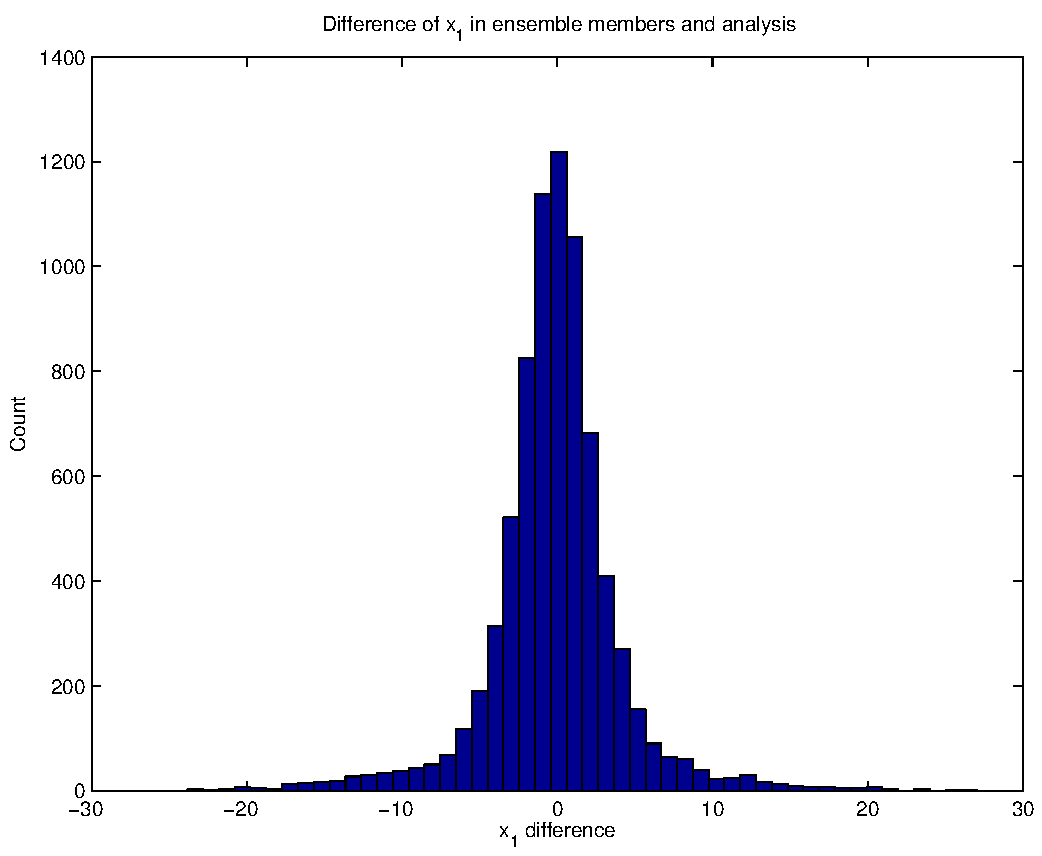
\includegraphics[width=0.45\textwidth]{figures/EnKF-histogram-analysis.pdf}
%%   \caption[The difference of ensemble forecasts from the analysis is reported for 760 assimilation windows in one model run of length 200, with 10 ensemble members and an assimilation window of length 0.261]{
%%     The difference of ensemble forecasts from the analysis is reported for 760 assimilation windows in one model run of length 200, with 10 ensemble members and an assimilation window of length 0.261.
%%     This has the same shape of as the difference between ensemble forecasts and the mean of the forecasts (not shown).
%%     This spread of ensemble forecasts is what allows us to estimate the error covariance of the forecast model, and appears to be normally distributed.
%%   }
%%   \label{fig:EnKFhist}
%% \end{figure}

The only difference between this approach and the EKF, in general, is that the forecast error covariance $\mbP^f$ is computed from the ensemble members, without the need for a tangent linear model:
\[ \mbP^f \approx \frac{1}{K-2} \sum _{k\neq l} \left ( \mbx_k ^f - \overline{\mbx} ^f _l \right ) \left (\mbx_k ^f - \overline{\mbx} ^f _l \right ) ^T .\]

The ETKF introduced by Bishop is one type of square root filter, and we present it here to provide background for the formulation of the LETKF \cite{bishop2001adaptive}.
For a square root filter in general, we begin by writing the covariance matrices as the product of their matrix square roots.
Because $\mbP_a,\mbP_f$ are symmetric positive-definite (by definition) we can write
\begin{equation} \mbP_a = \mbZ_a \mbZ_a^T ~~,~~~ \mbP_f = \mbZ_f \mbZ_f^T \end{equation}
for $\mbZ_a,\mbZ_f$ the matrix square roots of $\mbP_a,\mbP_f$ respectively.
We are not concerned that this decomposition is not unique, and note that $\mbZ$ must have the same rank as $\mbP$ which will prove computationally advantageous.
The power of the SRF is now seen as we represent the columns of the matrix $\mbZ_f$ as the difference from the ensemble members from the ensemble mean, to avoid forming the full forecast covariance matrix $\mbP_f$.
The ensemble members are updated by applying the model $M$ to the states $\mbZ_f$ such that an update is performed by
\begin{equation} \mbZ_f = M \mbZ_a .\end{equation}
To summarize, the steps for the ETKF are to (1) form $\mbZ_f^T\mbH^T\mbR^{-1}\mbH\mbZ_f$, assuming $\mathbf{R}^{-1}$ is easy, and (2) compute its eigenvalue decomposition, and apply it to $\mbZ_f$.

The LEKF implements a strategy that becomes important for large simulations: localization.
Namely, the analysis is computed for each grid-point using only local observations, without the need to build matrices that represent the entire analysis space.
This localization removes long-distance correlations from $\mathbf{B}$ and allows greater flexibility in the global analysis by allowing different linear combinations of ensemble members at different spatial locations \cite{kalnay20074}.
The general formulation of the LEKF by Ott \cite{ott2004local} goes as follows, quoting directly:
\begin{enumerate}
\item Globally advance each ensemble member to the next analysis timestep. Steps 2-5 are performed for each grid point
\item Create local vectors from each ensemble member
\item Project that point's local vectors from each ensemble member into a low dimensional subspace as represented by perturbations from the mean
\item Perform the data assimilation step to obtain a local analysis mean and covariance
\item Generate local analysis ensemble of states
\item Form a new global analysis ensemble from all of the local analyses
\item Wash, rinse, and repeat.
\end{enumerate}

Proposed by Hunt in 2007 with the stated objective of computational efficiency, the LETKF is named from its most similar algorithms from which it draws \cite{hunt2007efficient}.
With the formulation of the LEKF and the ETKF given, the LETKF can be  described as a synthesis of the advantages of both of these approaches.
This is the method that was sufficiently efficient for implementation on the full OpenFOAM CFD model of 240,000 model variables, and so we present it in more detail and follow the notation of Hunt et al (2007). 
As in the LEKF, we explicitly perform the analysis for each grid point of the model.
The choice of observations to use for each grid point can be selected a priori, and tuned adaptively.
Starting with a collection of background forecast vectors $\{ \mbx_{b(i)} \,:\,i=1..k \}$, we perform steps 1 and 2 in a global variable space, then steps 3-8 for each grid point:
\begin{enumerate}
\item apply $H$ to $\mbx_{b(i)}$ to form $\mby_{b(i)}$, average the $\mby_b$ for $\overline{\mby_b}$, and form $\mbY b$.
\item similarly form $\mbX_b$. (now for each grid point)
\item form the local vectors
\item compute $\mathbf{C}=(\mbY_b)^T\mbR^{-1}$ (perhaps by solving $\mbR \mathbf{C}^T = \mbY_b$
\item compute $\tilde{\mbP}_a = \left( (k-1)\mathbf{I} / \rho + \mathbf{C} \mbY _b \right ) ^{-1}$ where $\rho > 1$ is a tunable covariance inflation factor
\item compute $\mbW_a = \left ( (k-1) \tilde{\mbP} _a \right ) ^{1/2}$
\item compute $\overline{\mbw} _a  = \tilde{\mbP}_a \mathbf{C} \left ( \mby_o - \overline{\mby} _b \right )$ and add it to the column of $\mbW_a$
\item multiply $\mbX_b$ by each $\mbw_{a(i)}$ and add $\tilde{\mbx}_b$ to get $\left\{ \mbx_{a(i)}\,:\,i=1..k\right \}$ to complete each grid point
\item combine all of the local analysis into the global analysis
\end{enumerate}
The greatest implementation difficulty in the OpenFOAM model comes back to the spatial discretization and defining the local vectors for each grid point.

%% \begin{figure}[h!]
%%   \centering
%%   \includegraphics[width=0.45\textwidth]{../../2013/2013-05data-assimilation/src/experiments/DATest/DA_test_noname010.pdf}
%%   \caption[For near-perfect initial knowledge of the atmospheric state, the running average RMS error of a prediction using DA is compared against a prediction that does not]{
%%     For near-perfect initial knowledge of the atmospheric state, the running average RMS error of a prediction using DA is compared against a prediction that does not.
%%     Initial error for DA is normal with mean 0 and variance 0.01, and the RMS errors reported are averages of 3 runs.
%%     Observational noise is normally distributed with mean 0 and variance 0.05 (approximately 5\% of climatological variation), and an assimilation window length of 0.25 is used.
%%     As would be expected, in the long run DA greatly improves forecast skill, as forecasts without DA saturate to climatological error.
%%     The initial period where a forecast exceeds the skill of DA is potentially due to the spin-up time required by the filter to dial in the analysis error covariance.
%%   }
%%   \label{fig:DA_test}
%% \end{figure}

Next, we test the performance of each filter against increasing assimilation window length.
As we would expect, longer windows make forecasting more challenging for both algorithms.
The ensemble filter begins to out-perform the extended Kalman filter for longer window lengths because the ensemble more accurately captures the nonlinearity of the model.

\begin{figure}[h!]
  \centering
  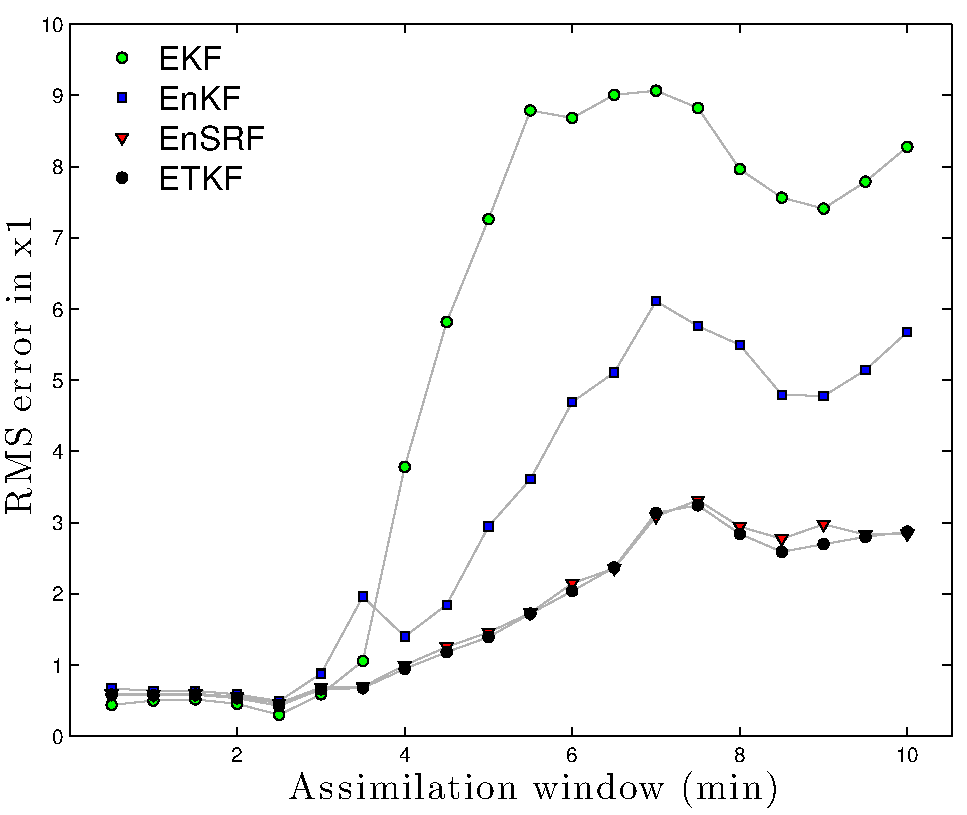
\includegraphics[width=0.45\textwidth]{figures/window_experiment_plot002.pdf}
  \caption[The RMS error is reported for our EKF and EnKF filters]{
    The RMS error (not scaled by climatology) is reported for our EKF and EnKF filters, measured as the difference between forecast and truth at the end of an assimiliation window for the latter 2500 assimiliation windows in a 3000 assimilation window model run.
    Error is measured in the only observed variable, $x_1$.
    Increasing the assimilation window led to an decrease in predictive skill, as expected.
    Additive and multiplicative covariance inflation is the same as Harris et. al (2011).
  }
  \label{fig:window_test}
\end{figure}

\begin{figure}[h!]
  \centering
  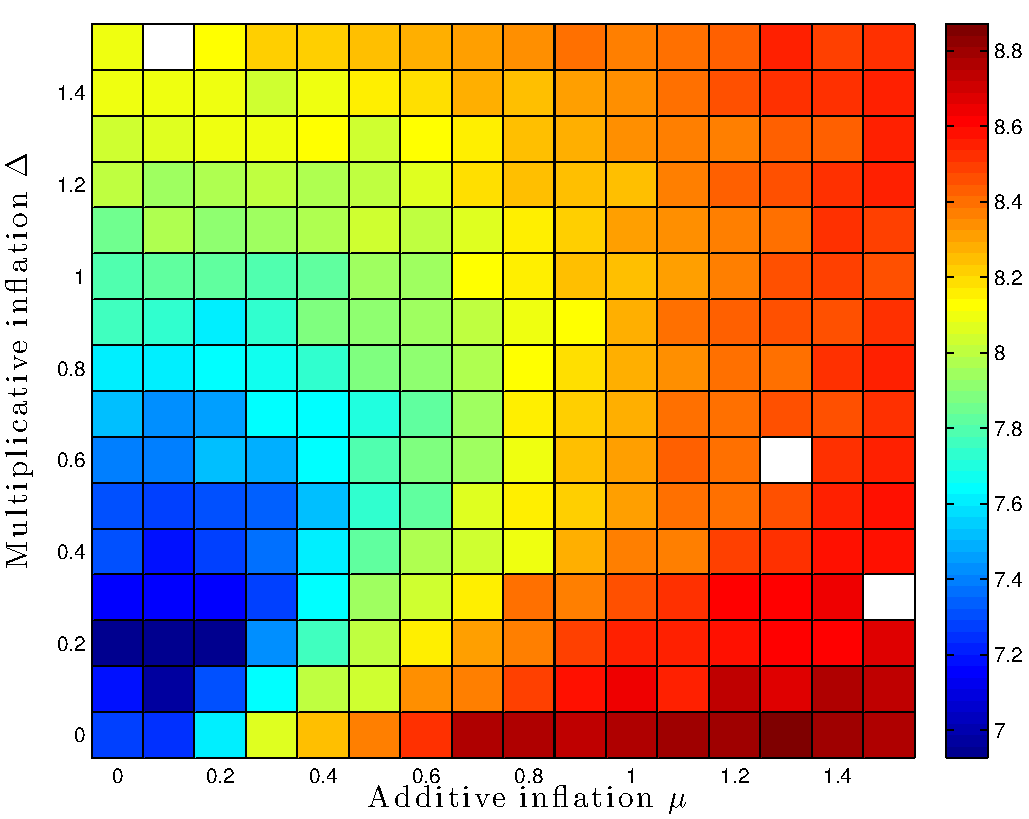
\includegraphics[width=0.45\textwidth]{figures/ETKF_390s_infl_error.pdf}
  \caption[The RMS error averaged over 100 model runs of length 1000 windows is reported for the ETKF for varying additive and multiplicative inflation factors]{
    The RMS error averaged over 100 model runs of length 1000 windows is reported for the ETKF for varying additive and multiplicative inflation factors $\Delta$ and $\mu$.
    Each of the 100 model runs starts with a random IC, and the analysis forecast starts randomly.
    The window length here is 390 seconds.
    The filter performance RMS is computed as the RMS value of the difference between forecast and truth at the assimilation window for the latter 500 windows, allowing a spin-up of 500 windows.
  }
  \label{fig:ETKF_cov_tuning_390s}

\end{figure}

\section{Results}

The first output of this work is a general data assimilation framework for MATLAB.
By utilizing an object-oriented (OO) design, the model and data assimilation algorithm code are separate and can be changed independently.
The principal advantage of this approach is the ease of incorporation of new models and DA techniques.

We first present the results pertaining to the accuracy of forecasts for synthetic data.
There are many possible experiments given the choice of assimilation window, data assimilation algorithm, localization scheme, model resolution, observational density, observed variables, and observation quality.
We focus on considering the effect of observations and observational locations on the resulting forecast skill.

In general, we see that increasing observational density leads to improved forecast accuracy.
With too few observations, the data assimilation is unable to recover the underlying dynamics.

\begin{figure}[h!]
  \centering
  \includegraphics[width=0.45\textwidth]{/Users/andyreagan/work/2013/2013-05data-assimilation/src/experiments/openFoamAssimilation/data/synData-tStep.01-b290-t340-m40000/results_vs_N_32_w10_labels.pdf}
  \caption[Prediction skill over time for synthetic temperature sensors]{
    Prediction skill over time for synthetic temperature sensors.
    With these observations, our DA scheme is unable to predict the model run at all.
    Compared with operational NWP, we are observing far less model variables in this situation, with $10^5$ times more model variables than observations, even for the 32 sensors.
  }
  \label{fig:TsensorExp}
\end{figure}

While the inability to predict the flow direction with these synthetic temperature sensors may cast doubt on the possibility of predicting a physical experiment using CFD, we discuss improvements to our prediction system that may be able to overcome these initial difficulties.
Regardless, in Figure \ref{fig:fullObsExp} we verify directly that our assimilation procedure is working adequately with a sufficient number of observations: temperature at all cells.

\begin{figure}[h!]
  \centering
  \includegraphics[width=0.45\textwidth]{/Users/andyreagan/work/2013/2013-05data-assimilation/src/experiments/openFoamAssimilation/data/synData-tStep.01-b290-t340-m40000/results_vs_N_40000_w10_labels.pdf}
  \caption[Prediction skill over time for complete observations of temperature]{
    Prediction skill over time for complete observations of temperature.
    With these observations, our DA scheme is able to predict the model run well.
    Increasing the number of ensemble members $N$ leads to a decrease in the forecast error, as one would hope with a more complete sampling of model uncertainty.
    Note that although we may full observations of temperature, it is only one of five model variables assimilated.
  }
  \label{fig:fullObsExp}
\end{figure}

Beyond real-time prediction, it is now possible to design and test new methods of data assimilation for large scale systems.
New methods specific to CFD, possibly using principle mode decomposition of flow fields have the potential to greatly improve the skill of real-time CFD applications.
In Figure \ref{fig:localcovadaptive}, flow structures present in our computational experiment demonstrate the potential for adaptive covariance localization.

The numerical coupling of CFD to experiment by DA should be generally useful to improve the skill of CFD predictions in even data-poor experiments, which can provide better knowledge of unobservable quantities of interest in fluid flow.


